\chapter{Implementation and experiments}
\label{implementation_and_experiments}

\section{Performance analysis}
To observe the current situation, we have measured Tribler running idle (i.e. no human interaction) for 4 hours.
For this experiment we run Tribler version 6.6.0-exp1 which is a pre-release of 6.6, because it includes the MultiChain code.
The hardware used during this experiment can be seen in Table \ref{table:tribler_idle}.

\begin{table}[h]
	\centering
	\begin{tabular}{l|l}
		\textbf{Component} 	& \textbf{Specifications} \\ \hline
		Operating System   	& Ubuntu 16.04 LTS \\
		Python version		& 2.7.12 \\
		CPU					& Intel Core i5-2410M \\ 
		HDD					& Samsung 850 EVO 250GB  \\ 
		RAM					& 8 GB DDR3 1600MHz \\
	\end{tabular}
	\caption{Specifications of the setup used during the idle iotop measurement of Tribler 6.6.0-pre-exp.}
	\label{table:tribler_idle}
\end{table}

\begin{figure}[h]
	\makebox[\textwidth][c]{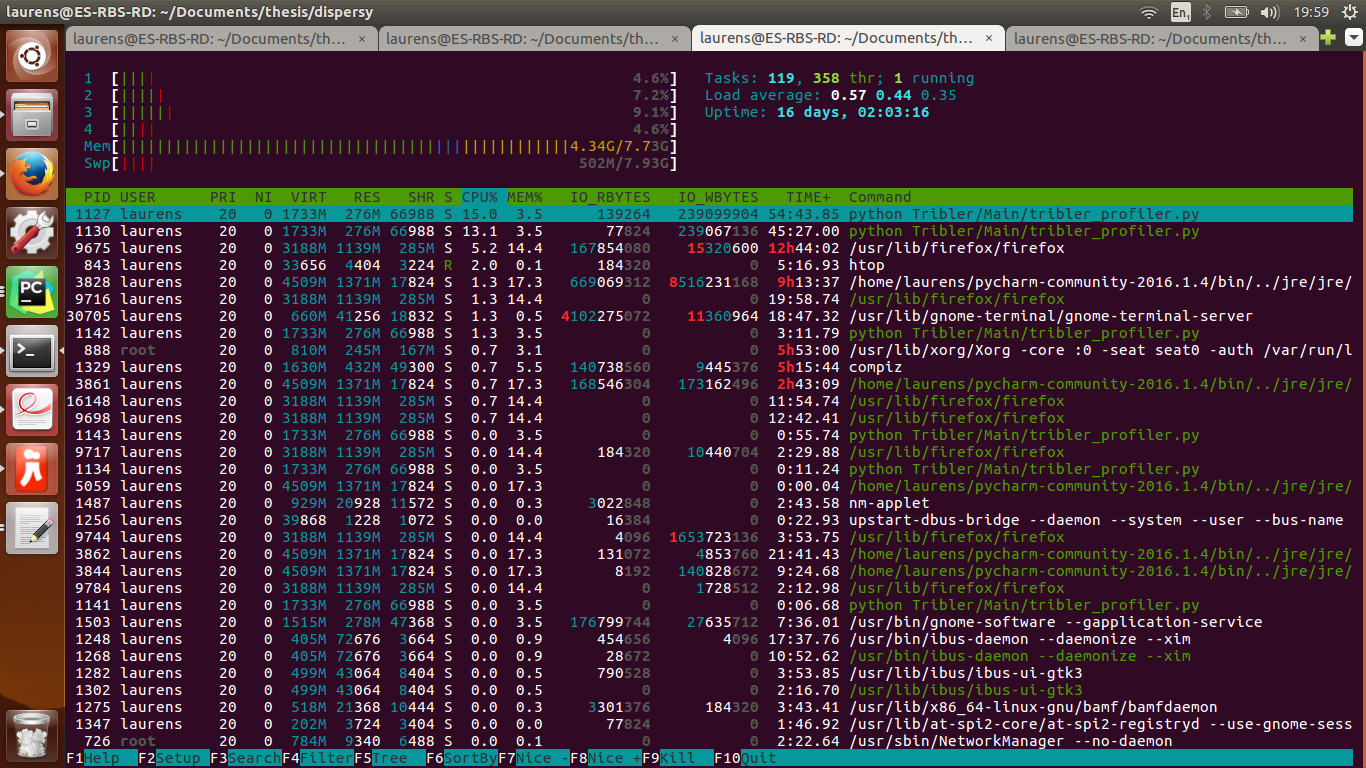
\includegraphics[width=0.95\paperwidth]{experimentation/images/htop.png}}
	\caption{The output of a four hour idle run.}
	\label{fig:htop_io_idle_run}
\end{figure} 

The results are visible in Figure~\ref{fig:htop_io_idle_run}. \todo{cut unity desktop}
From these results we observe that Tribler current has an IO of 144 MB/Hour.
To observe the individual components separately, we have created a breakdown the database queries performed by Tribler.
This breakdown is visible in Table Z.
As we can see, B is doing the most IO... \todo{Implement breakdown functionality and measure this.}

\section{Validating the performance regression system}

To validate the performance regression system, we have resolved one of Tribler's biggest bottlenecks: Dispersy's database I/O.
Dispersy performs a lot of I/O.
Currently, this I/O is blocking the main thread when waiting for the database, wasting valuable CPU cycles.
To address this problem, we have written Dispersy's I/O to become asynchronous and non-blocking.
To realize this, a new database manager \enquote{StormDBManager} is introduced and 90\%\todo{made up number, need to calculate the actual value.} of Dispersy's functions have been refactored.

